%%%%%%%%%%%%%%%%%%%%%%%%%%%%%%%%%%%%%%%%%%%%%%%%%%%%%%%%%%%%%%%%%%%%
%% I, the copyright holder of this work, release this work into the
%% public domain. This applies worldwide. In some countries this may
%% not be legally possible; if so: I grant anyone the right to use
%% this work for any purpose, without any conditions, unless such
%% conditions are required by law.
%%%%%%%%%%%%%%%%%%%%%%%%%%%%%%%%%%%%%%%%%%%%%%%%%%%%%%%%%%%%%%%%%%%%

\documentclass[
  digital, %% This option enables the default options for the
           %% digital version of a document. Replace with `printed`
           %% to enable the default options for the printed version
           %% of a document.
  twoside, %% This option enables double-sided typesetting. Use at
           %% least 120 g/m² paper to prevent show-through. Replace
           %% with `oneside` to use one-sided typesetting; use only
           %% if you don’t have access to a double-sided printer,
           %% or if one-sided typesetting is a formal requirement
           %% at your faculty.
  table,   %% This option causes the coloring of tables. Replace
           %% with `notable` to restore plain LaTeX tables.
  nolof,     %% This option prints the List of Figures. Replace with
           %% `nolof` to hide the List of Figures.
  nolot,     %% This option prints the List of Tables. Replace with
           %% `nolot` to hide the List of Tables.
  %% More options are listed in the user guide at
  %% <http://mirrors.ctan.org/macros/latex/contrib/fithesis/guide/mu/fi.pdf>.
]{fithesis3}
\usepackage{gensymb}
\usepackage{subcaption}
%% The following section sets up the locales used in the thesis.
\usepackage[resetfonts]{cmap} %% We need to load the T2A font encoding
\usepackage[T1,T2A]{fontenc}  %% to use the Cyrillic fonts with Russian texts.
\usepackage[
  main=slovak, %% By using `czech` or `slovak` as the main locale
                %% instead of `english`, you can typeset the thesis
                %% in either Czech or Slovak, respectively.
  english, german, russian, czech, slovak %% The additional keys allow
]{babel}        %% foreign texts to be typeset as follows:
%%
%%   \begin{otherlanguage}{german}  ... \end{otherlanguage}
%%   \begin{otherlanguage}{russian} ... \end{otherlanguage}
%%   \begin{otherlanguage}{czech}   ... \end{otherlanguage}
%%   \begin{otherlanguage}{slovak}  ... \end{otherlanguage}
%%
%% For non-Latin scripts, it may be necessary to load additional
%% fonts:
\usepackage{paratype}
\def\textrussian#1{{\usefont{T2A}{PTSerif-TLF}{m}{rm}#1}}
%%
%% The following section sets up the metadata of the thesis.
\thesissetup{
    date          = \the\year/\the\month/\the\day,
    university    = mu,
    faculty       = fi,
    type          = bc,
    author        = Henrieta Micheľová,
    gender        = f,
    advisor       = prof. RNDr. Ivana Černá{,} CSc.,
    title         = {Distribuované algoritmy pro rekonfiguraci platformy RoFI},
    TeXtitle      = {Distribuované algoritmy pro rekonfiguraci platformy RoFI},
    keywords      = {RoFI platforma, MPI, ...},
    TeXkeywords   = {RoFI platforma, MPI, \ldots},
    abstract      = {This is the abstract of my thesis, which can

                     span multiple paragraphs.},
    thanks        = {These are the acknowledgements for my thesis, which can

                     span multiple paragraphs.},
    bib           = bibliography.bib,
}
\usepackage{makeidx}      %% The `makeidx` package contains
\makeindex                %% helper commands for index typesetting.
%% These additional packages are used within the document:
\usepackage{paralist} %% Compact list environments
\usepackage{amsmath}  %% Mathematics
\usepackage{amsthm}
\usepackage{amsfonts}
\usepackage{url}      %% Hyperlinks
\usepackage{markdown} %% Lightweight markup
\usepackage{listings} %% Source code highlighting
\lstset{
  basicstyle      = \ttfamily,%
  identifierstyle = \color{black},%
  keywordstyle    = \color{blue},%
  keywordstyle    = {[2]\color{cyan}},%
  keywordstyle    = {[3]\color{olive}},%
  stringstyle     = \color{teal},%
  commentstyle    = \itshape\color{magenta}}
\usepackage{floatrow} %% Putting captions above tables
\floatsetup[table]{capposition=top}
\begin{document}
\chapter*{Úvod}
\addcontentsline{toc}{chapter}{Úvod}

\chapter{Popis platformy RoFI}
\label{sec:platform}
RoFI je modulárna robotická platforma, ktorá vzniká na pôde Fakulty informatiky Masarykovej univerzity v laboratóriu ParaDiSe\footnote{Laboratoř paralelních a distribuovaných systémů (stránka laboratória: \url{https://paradise.fi.muni.cz/})}. Táto platforma zastrešuje vývoj modulárnych robotov a iného príslušenstva po ich hardvérovej, ale aj softvérovej stránke na rôznych úrovniach. 

Primárnym cieľom platformy RoFI je vytvorenie modulárnych robotov, ktoré je možné využiť na rôzne úlohy. Príkladom sú úlohy ako prechádzanie cez úzke priestory, prekonávanie prekážok a podobne. 

Ich dizajn je navrhovaný tak, aby bolo jednoduché a nie príliš finančne náročné ich fyzicky skonštruovať. Softvérové vybavenie pokrýva široké spektrum požiadaviek modulárnych robotov a je jednoduché na prácu aj menej skúseným užívateľom. Zároveň je platforma navrhnutá tak, aby bola ľahko rozšíriteľná o dodatočné periférie a pasívne prvky. 

Základnou jednotkou platformy RoFI sú moduly \cite{mrazekMasterThesis}, ktoré sú schopné sa vzájomne fyzicky prepojiť a zároveň medzi sebou komunikovať \cite{rofiCom}. Okrem toho sa každý modul dokáže pripojiť aj na pasívne prvky. 

Prepojenie viacerých modulov umožňuje vytvoriť tzv. RoFIbotov \cite{rofiWeb}, ktoré majú širšie spektrum funkcionalít ako samostatné moduly. Cieľom tejto práce je práve zamerať sa na RoFIbotov a ich schopnosť rekonfigurovať sa za špecifických podmienok (podrobnejší popis v kapitole \ref{sec:restrictions}). 

Pre účel tejto práce je v kapitole \ref{sec:moduleSpec} popísaná iba časť hardvérového vybavenia modulu a schopnosti prepájania modulov. Ďalšie rozšírenia, softvérové vybavenie a iné komponenty a návody sa nachádzajú na stránkach platformy \cite{rofiWeb}. 

\section{Formálna špecifikácia modulov}
\label{sec:moduleSpec}
Modul platformy RoFI bol navrhnutý tak, aby bol tzv. \textit{lattice type}\footnote{každý modul je umiestnený v pravidelnej 3D mriežke} a zároveň má vlastnosť \textit{grid-awareness}\footnote{pri pohybe modulu zasahuje modul do najnižšieho počtu polí mriežky}. V súčasnej dobe je platforma RoFI prispôsobená na mriežku s veľkosťou 10\,cm. Podrobný popis vlastností sa nachádza v diplomovej práci \textit{RoFI – Distributed Metamorphic Robots} \cite{mrazekMasterThesis}. 

\begin{figure}[hbt!]
    \centering
    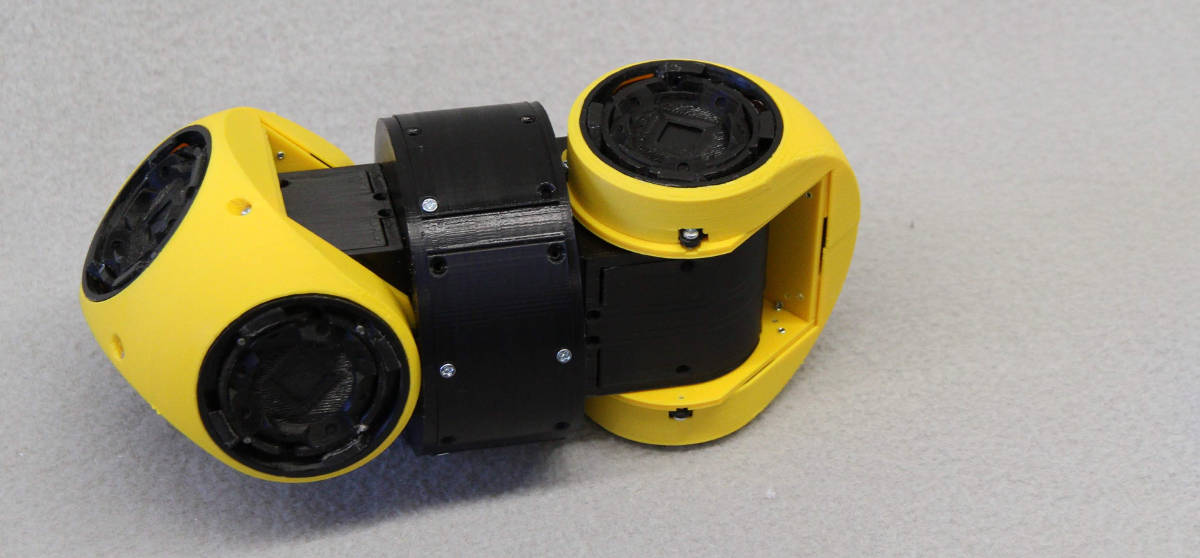
\includegraphics[width=0.6\textwidth]{pictures/module.jpg}
    \caption[Fotografia modulu]{Fotografia univerzálneho modulu \cite{rofiWeb}.}
    \label{fig:module}
\end{figure}

Každý z modulov sa skladá z dvoch častí (\textit{side A} a \textit{side B}). Každá z nich sa delí na dve časti označené ako \textit{body} a \textit{shoe} (viď obrázok \ref{fig:module_parts}). 

\begin{figure}[hbt!]
    \centering
    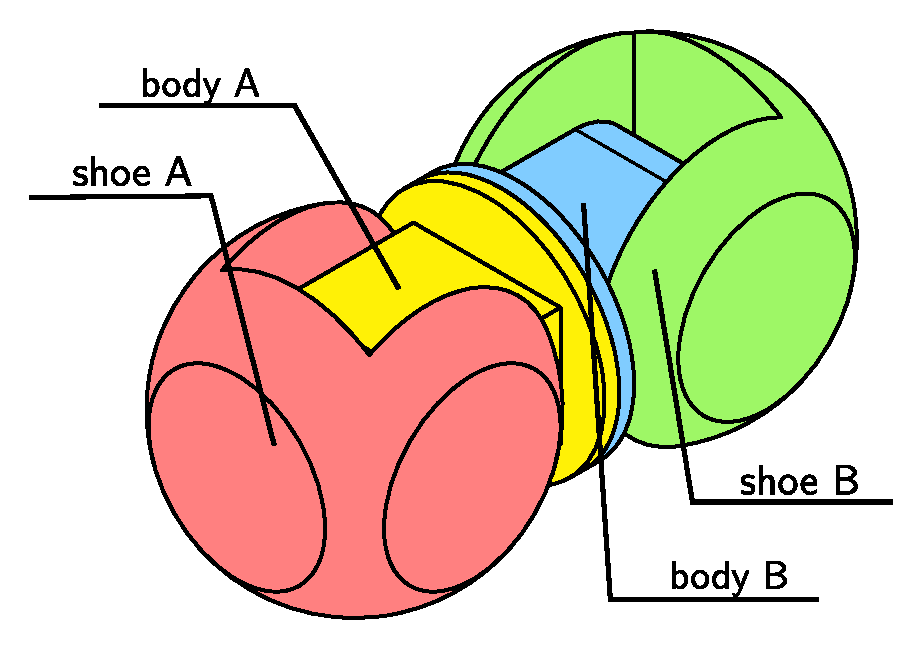
\includegraphics[width=0.6\textwidth]{pictures/module_parts.pdf}
    \caption[Časti modulu]{Schéma častí modulu \cite{mrazekMasterThesis}.}
    \label{fig:module_parts}
\end{figure}

Moduly majú schopnosť sa pohybovať, a to vďaka až trom stupňom voľnosti. Prvé dva z nich umožňujú pohybovať so \textit{shoe} časťou modulu. Konkrétne ide o pohyb okolo osí označovaných ako $\alpha$ a $\beta$  o uhol v rozsahu $\interval[{-90\degree, 90\degree}]$. Posledným stupňom voľnosti je pohyb okolo osi označovanej ako $\gamma$. Tento pohyb umožňuje otáčaním meniť vzájomnú polohu \textit{body} častí modulu a jeho rozsah je $\interval({-180\degree, 180\degree}]$. 

\begin{figure}[hbt!]
    \centering
    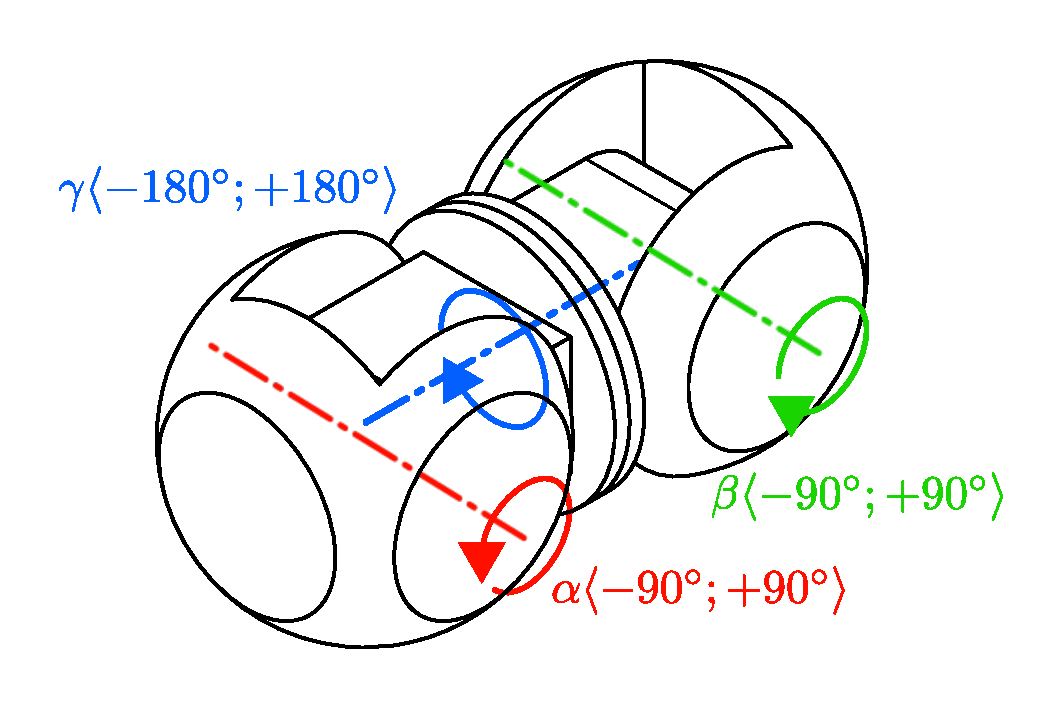
\includegraphics[width=0.6\textwidth]{pictures/module_angles.pdf}
    \caption[Stupne voľnosti modulu]{Schéma stupňov voľnosti modulu a smerov otáčania \cite{mrazekMasterThesis}.}
    \label{fig:module_angle}
\end{figure}

Ako bolo spomenuté vyššie, tak každý modul má schopnosť pripojiť sa k iným modulom (a vytvoriť tak RoFIbotov) alebo k pasívnym prvkom pomocou dockov. Dockovací systém platformy RoFI je navrhnutý ako tzv. \textit{genderless}, čo umožňuje vzájomné spojenie ľubovoľných dvoch dockov. 

Každý modul obsahuje práve šesť dockov, ktoré sú rozmiestnené po tri na každej \textit{shoe} modulu. Dock je okrem svojej polohy na module definovaný aj orientačným vektorom (viď obrázok \ref{fig:dock_desc}). 

\begin{figure}[hbt!]
    \centering
    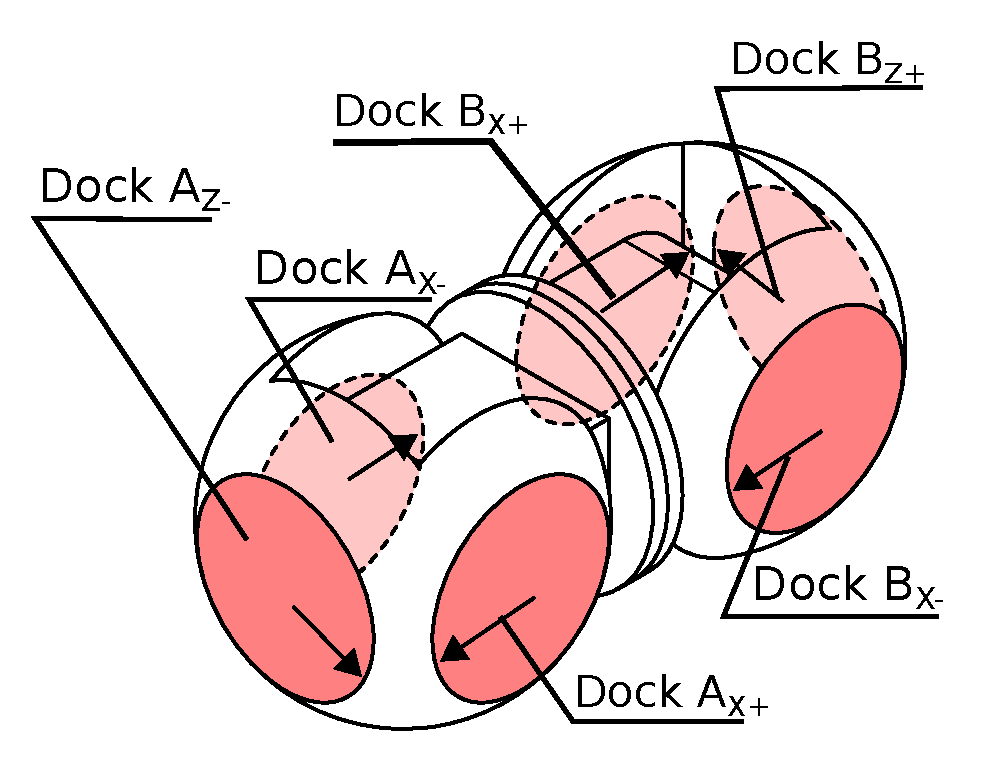
\includegraphics[width=0.6\textwidth]{pictures/dock_desc.pdf}
    \caption[Docky modulu]{Schéma umiestnení dockov na module a ich označenia. Šípky na dockoch znázorňujú orientačné vektory \cite{mrazekMasterThesis}.}
    \label{fig:dock_desc}
\end{figure}

Prepojenie je definované vzájomnou polohou orientačných vektorov dockov spojenia. Konštrukcia dockov dovoľuje ich prepojenie až v štyroch rôznych polohách. 

Vzájomná poloha orientačných vektorov dockov môže byť postupne $0\degree$, $90\degree$, $180\degree$ alebo $270\degree$ a tieto prepojenia sa označujú v tomto poradí ako \textit{North}, \textit{East}, \textit{South} a \textit{West} (viď obrázok \ref{fig:dock_orientation}). 

\begin{figure}[hbt!]
    \centering
    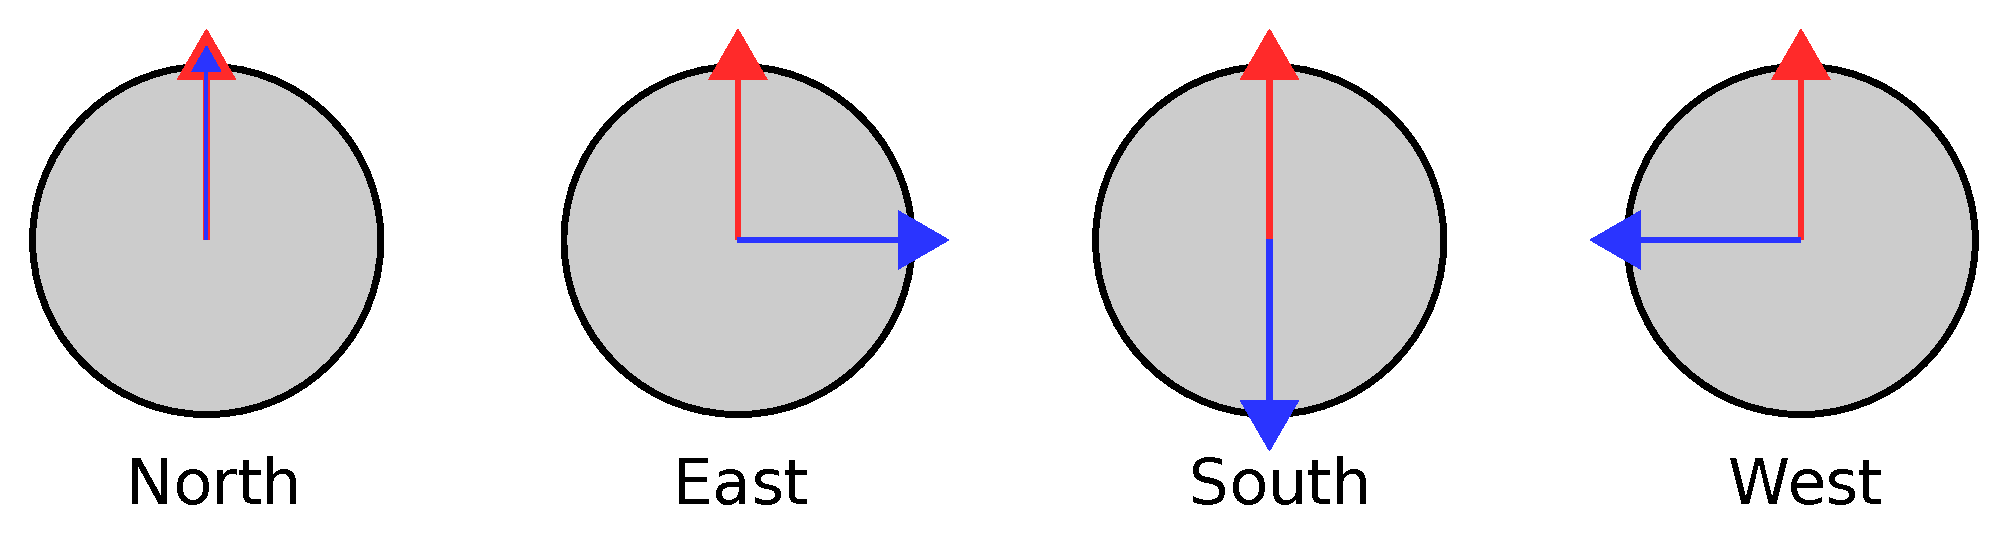
\includegraphics[width=0.6\textwidth]{pictures/dock_orientation.pdf}
    \caption[Poloha prepojenia dockov modulu]{Schéma vzájomnej polohy orientačných vektorov spojených dockov modulov. Červenou je označený dock modulu, z ktorého perspektívy spojenie označujeme. Modrá šípka je orientačný vektor druhého modulu. Poznámka: nezáleží na výbere docku, z ktorého perspektívy spojenie sledujeme \cite{mrazekMasterThesis}.}
    \label{fig:dock_orientation}
\end{figure}

\section{Špecifikácia RoFIbotov}
\label{sec:rofibotSec}
Vzájomné prepojenie modulov pomocou dockov vytvára RoFIbotov. Parametre RoFIbota, ktoré ho definujú, sa dajú rozdeliť do dvoch kategórií:   
\begin{enumerate}
    \item tvar RoFIbota vzhľadom na jeho vnútornú štruktúru: 
    \begin{itemize}
        \item množina modulov RoFIbota, 
        \item množina prepojení (hrán) modulov; 
    \end{itemize}
    \item poloha RoFIbota vzhľadom k okolitému svetu: 
    \begin{itemize}
        \item natočenie celého RoFIbota vzhľadom na okolie, 
        \item umiestnenie RoFIbota do priestoru.  
    \end{itemize}
\end{enumerate}

\textit{Konfigurácia} RoFIbota je tvar RoFIbota vzhľadom na jeho vnútornú štruktúru, teda množina modulov a ich prepojení. 

Každý modul v konfigurácii RoFIbota je definovaný jedinečným identifikátorom modulu a hodnotami všetkých troch stupňov voľnosti modulu. 

Jednotlivé hrany (prepojenia) v konfigurácii RoFIbota sú definované identifikátormi spojených modulov a presným popisom dockov, ktorými sú prepojené a vzájomnou polohou spojených dockov. 

Formálne značenie všetkých parametrov konfigurácie a ich rozsahy sú zavedené v kapitole \ref{sec:inputOutput}. 

\textit{Rekonfigurácia} RoFIbota je postupnosť validných krokov (ich zoz\-nam a formálna definícia sa nachádza v kapitole \ref{sec:reconfigActions}), ktorá umožní zmeniť počiatočnú konfiguráciu RoFIbota na cieľovú konfiguráciu RoFIbota. 

\section{Formulácia problému}
\label{sec:restrictions}
Cieľom tejto práce je navrhnúť a implementovať algoritmy na rekonfiguráciu RoFIbotov, ktoré spĺňajú podmienky popísané v tejto kapitole a následne evaluovať výsledky. 

Pre účely tejto práce je zavedený predpoklad, že RoFIboti nemajú definované natočenie a umiestnenie do okolitého sveta. Tým pádom je postačujúce, že RoFIbot je definovaný iba svojou konfiguráciou. 

Každý RoFIbot vykonáva svoju rekonfiguráciu „vo vákuu“, bez fyzických obmedzení reálneho sveta (ako je napríklad podlaha, či iné prekážky). Zároveň fyzikálne zákony (napríklad gravitácia) pri rekonfigurácii nehrajú žiadnu rolu. 

Zároveň musí platiť, že v každom kroku rekonfigurácie musí byť RoFIbot vo validnej konfigurácii, čo napríklad značí, že nesmie dôjsť ku kolíziám modulov (konkrétny popis v kapitole \ref{sec:reconfigActions}). 

Keďže komunikácia medzi modulmi môže prebiehať po fyzickom spojení pomocou dockov, ale aj bezdrôtovo, tak si zadefinujeme spojitosť RoFIbota. 

\begin{figure}[hbt!]
    \centering
    \begin{subfigure}[b]{0.49\textwidth}
        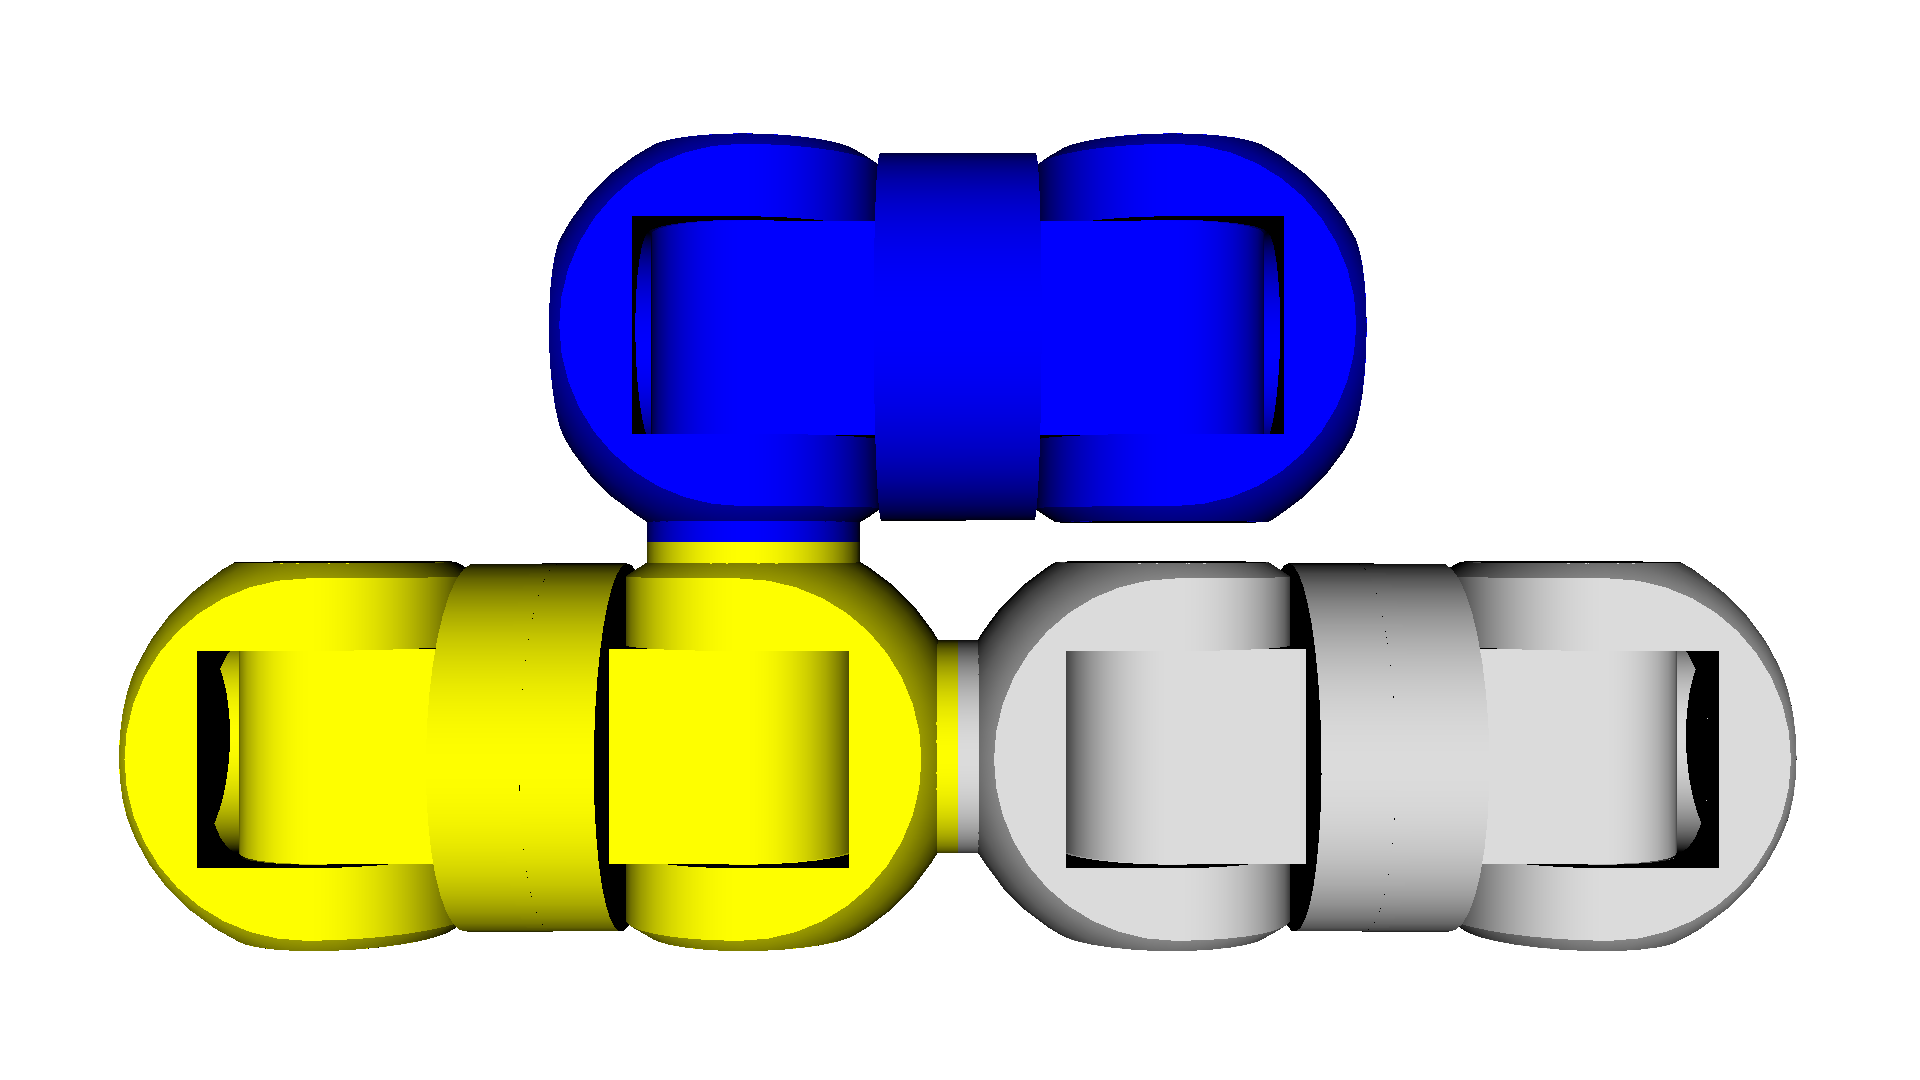
\includegraphics[width=\textwidth]{pictures/connected_rofibot.png}
        \caption[Spojitá konfigurácia.]{Spojitá konfigurácia}
        \label{fig:connectCfg}
    \end{subfigure}
    \begin{subfigure}[b]{0.49\textwidth}
        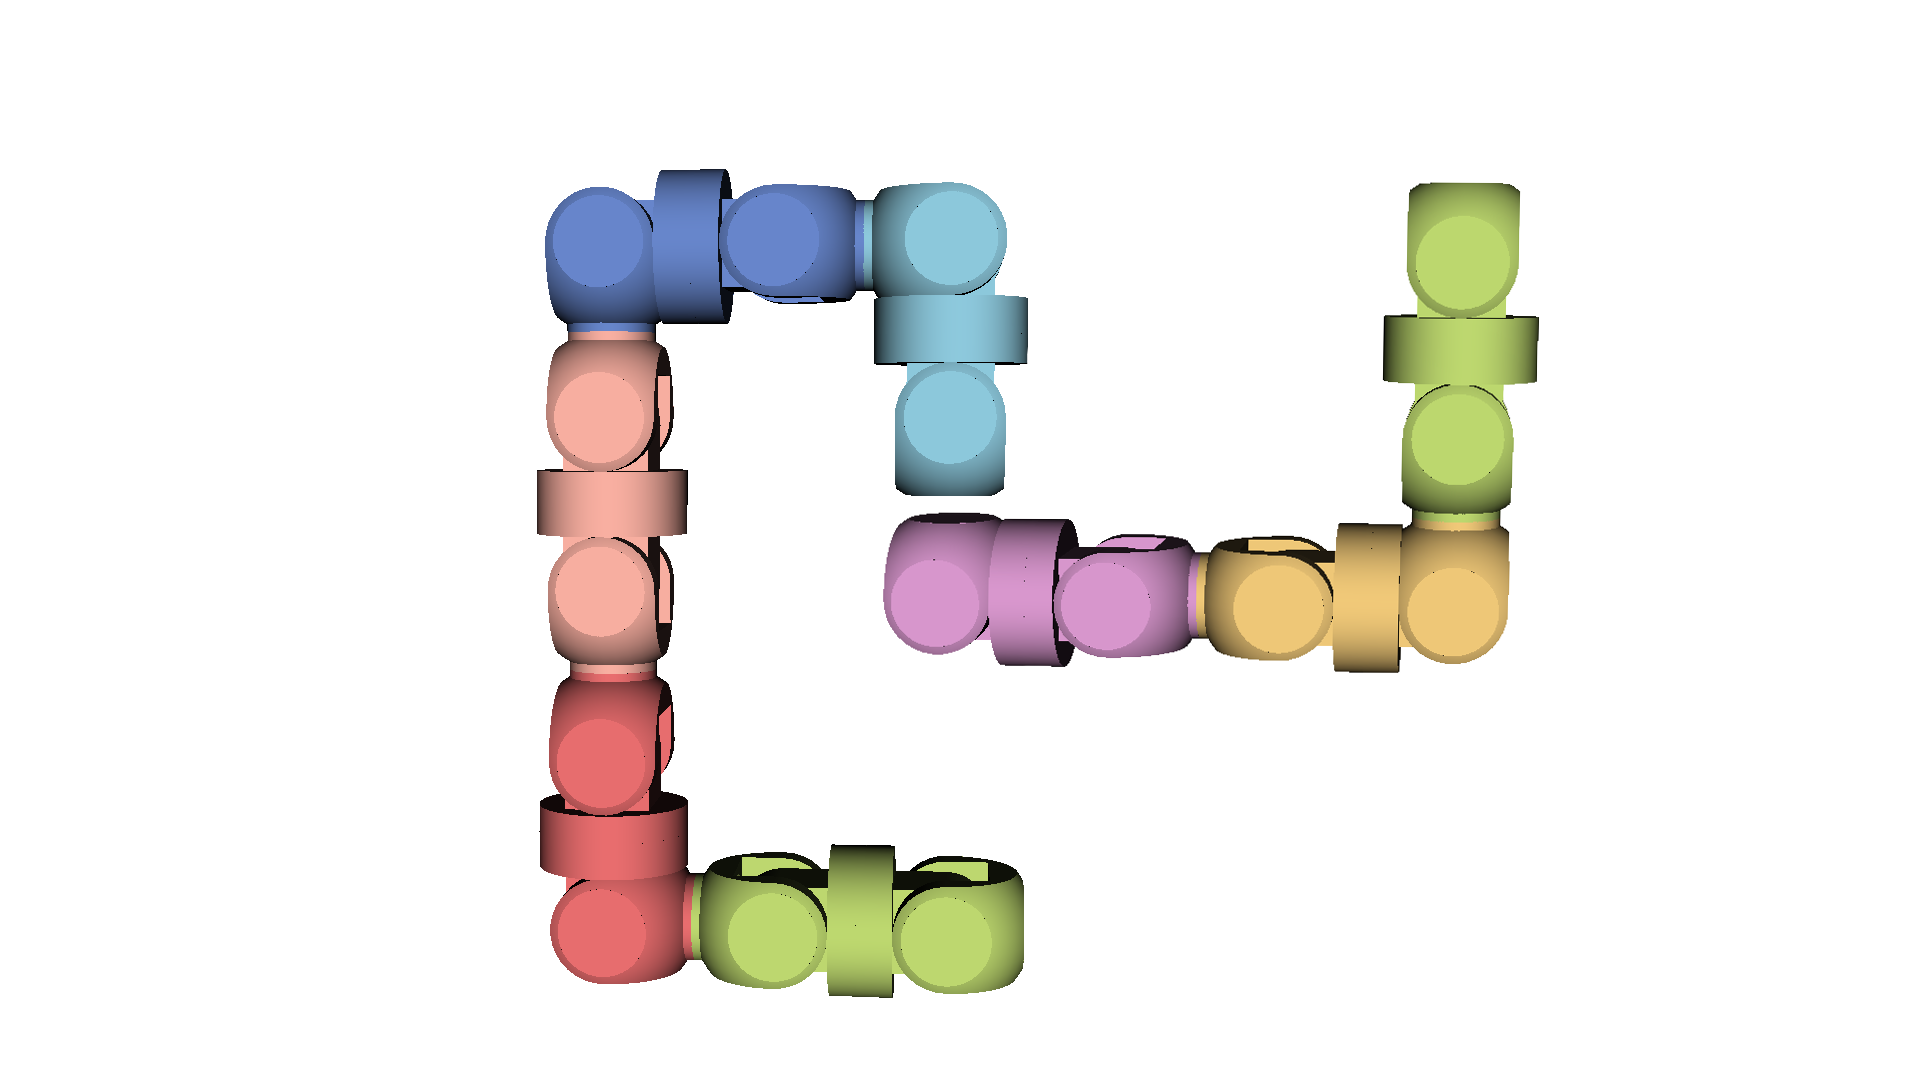
\includegraphics[width=\textwidth]{pictures/disconneted_rofibot.png}
        \caption[Nespojitá konfigurácia.]{Nespojitá konfigurácia}
        \label{fig:disconnectCfg}
    \end{subfigure}
    \caption[Príklad konfigurácie]{Príklad spojitej a nespojitej konfigurácie.}
    \label{fig:exampleCfg}
\end{figure}

RoFIbot je \textit{spojitý}, ak medzi akýmikoľvek jeho dvomi modulmi RoFIbota existuje cesta tvorená modulmi a prepojeniami. To značí, že komunikácia medzi akýmikoľvek dvomi modulmi spojitého RoFIbota môže prebiehať výhradne fyzickými spojeniami (viď príklad spojitej a nespojitej konfigurácie na obrázku \ref{fig:exampleCfg}). 

V rámci tejto práce je zavedený predpoklad, že RoFIbot, ktorý sa rekonfiguruje, je v počiatočnej konfigurácii, počas celého procesu rekonfigurácie, ale aj v cieľovej konfigurácii spojitý. 

\chapter{Distribuované algoritmy}
\label{sec:distributedAlgo}
Obsahom tejto kapitoly je formálna špecifikácia konfigurácie RoFIbota a prípustných akcií použiteľných na rekonfiguráciu. Popis samotných algoritmov sa nachádza v kapitole \ref{sec:algoDesc}. 

Diplomová práca \textit{Motion Planning for the RoFI Platform} \cite{vozarovaMasterThesis} popisuje rekonfiguráciu RoFIbotov z centralizovaného pohľadu, teda s úplnou znalosťou počiatočnej a cieľovej konfigurácie RoFIbota. 

Platforma RoFI je však navrhnutá ako distribuovaný systém, kde najmenšou stavebnou jednotkou je modul. Z toho vyplýva, že RoFIbot nemá žiadnu centralizovanú logickú jednotku, ktorá by dokázala riadiť rekonfiguráciu. 

Distribuované algoritmy na rekonfiguráciu sú navrhnuté tak, aby každý z modulov s rovnakou verziou algoritmu dokázal zo svojich vstupných údajov (popis v kapitole \ref{sec:inputOutput}) pomocou posielania si správ medzi ostatnými modulmi RoFIbota vykonať jeho rekonfiguráciu. 

Samotný modul nepozná celú konfiguráciu RoFIbota (dokonca pri veľkých konfiguráciách by znalosť celej konfigurácie mohla zberať veľa miesta v pamäti a nebola by potrebná). V tejto práci má každý modul znalosť výhradne o svojom stave. Každý ďalší údaj o stave iných modulov vie získať výhradne posielaním si správ. 

\textit{Stav modulu} je tvorený nasledujúcimi údajmi: unikátny identifikátor modulu, aktuálne hodnoty natočenia stupňov voľnosti modulu a kompletná informácia o všetkých prepojeniach daného modulu. 

\section{Formálna špecifikácia konfigurácie}
\label{sec:inputOutput}
--- poznamky

Navrhnuté vstupné a výstupné údaje konfigurácie RoFIbota a prípustných akcií na rekonfiguráciu sú prevzaté z diplomovej práce \textit{Motion Planning for the RoFI Platform} \cite{vozarovaMasterThesis}. 

\cite{nausovaBachelorThesis}

vstupné a výstupné údaje + kompatibilita s vizualizérom

\section{Špecifikácia rekonfigurácie RoFIbota}
\label{sec:reconfigActions}


\chapter{Implementácia}
\label{sec:implementation}
\section{Technická špecifikácia a využité knižnice}
\label{sec:libraries}
\section{Popis algoritmov na rekonfiguráciu}
\label{sec:algoDesc}
\subsection{Centralizovane-distribuovaný algoritmus - //TODO premenovat}
\subsection{Distribuovaný algoritmus}

\chapter{Experimentálne zhodnotenie}
\section{Ukážkové rekonfigurácie}
Ukážkové konfigurácie a porovnanie rýchlostí ich výpočtov a prípadne rôznorodosti nájdených riešení

Odkazy na videá, obrázky, presné časy behov a rôznosť riešení. 
\section{Evaluácia výsledkov na vzorových príkladoch}
Porovnanie algoritmov z pohľadu časovej a priestorovej zložitosti

Popis, ktorý algoritmus a na aké konfigurácie a zmeny v rekonfiguráciách je viac vhodný

\chapter{Záver}
Rekapitulácia. 
Ako ďalej zlepšovať algoritmy a čo ešte pridávať a podobne. 

%\listoffigures
  \printbibliography[heading=bibintoc] %% Print the bibliography.


\end{document}
